\documentclass{beamer}
\usepackage[english]{babel}
\usepackage{color}
\usepackage{amsfonts}
\usepackage{amssymb}
\usepackage{epsfig}
\usepackage{amsmath}
\usepackage{txfonts}
\usepackage{relsize}
\usepackage{physics}
\usepackage{natbib}
\usepackage{bibentry}
\bibliographystyle{apalike}
\usepackage{tikz}
\usepackage{ifthen}
\usetikzlibrary{decorations.pathreplacing}

\newcommand\footcite[1]{\footnote{\bibentry{#1}}\label{\thepage:#1}}
\newcommand\secondcite[1]{\textsuperscript{\ref{\thepage:#1}}}

%\usepackage{bbold}
\usepackage{dsfont}
\usepackage{bbm}

\usepackage[latin1]{inputenc}

\newcommand{\id}{\mathbbm{1}}
\newcommand{\HH}{\mathcal{H}}
\newcommand{\CC}{\mathbb{C}}
\newcommand{\BB}{\mathcal{B}}
\newcommand{\UU}{\mathcal{U}}
\newcommand{\ZZ}{\mathbb{Z}}
\renewcommand{\AA}{\mathcal{A}}
\newcommand{\Ad}[1]{\textrm{Ad}\left(#1\right)}

\newcommand{\mean}[1]{\langle #1 \rangle}
\newcommand{\cumul}[1]{\langle\!\langle #1 \rangle\!\rangle}

\renewcommand{\d}{\textrm{d}}

\DeclareRobustCommand{\augiefamily}{%
	\fontfamily{augie}\fontseries{m}\fontshape{n}\selectfont}
\DeclareTextFontCommand{\textaugie}{\augiefamily}


\setbeamertemplate{caption}{\raggedright\insertcaption\par}

\mode<presentation>
{
	\usetheme{CambridgeUS}
	
	\setbeamercovered{transparent}
}


\definecolor{Or}{RGB}{255,153,000}
\definecolor{Indigo}{RGB}{72,61,139}
\definecolor{Magenta}{RGB}{139,0,139}

\setbeamercolor{normal text}{fg=black,bg=white}
\setbeamercolor{alerted text}{fg=Indigo}
\setbeamercolor{example text}{fg=Indigo}

%\setbeamercolor{background canvas}{fg=myforeground, bg=white}
%\setbeamercolor{background}{fg=myforeground, bg=mybackground}
%
%\setbeamercolor{palette primary}{fg=black, bg=gray!30!white}
%\setbeamercolor{palette secondary}{fg=black, bg=gray!20!white}
%\setbeamercolor{palette tertiary}{fg=black, bg=gold}



\setbeamercolor{palette tertiary}{fg=black, bg=Indigo}
\setbeamercolor{frametitle}{fg=Indigo}
\setbeamercolor{title}{fg=Indigo}
\setbeamercolor{footline}{fg=Indigo, bg=Indigo}
\setbeamercolor{author in head/foot}{fg=black}
\setbeamercolor{date in head/foot}{fg=black}
\setbeamercolor{title in head/foot}{fg=black}

\definecolor{Highlight}{RGB}{139,0,139}
\newcommand{\HL}[1]{{\color{Highlight}#1}}

\usefonttheme{professionalfonts}
\beamertemplatenavigationsymbolsempty

\setlength{\parskip}{0.1cm}

\title[SPT classification]%\hspace{1cm} \insertframenumber/\inserttotalframenumber]
{Topological phases of matter:\\From the quantum hall effect to symmetry protected topological order}

\author[Tijl Jappens]
{Tijl Jappens \\
 \scriptsize KU Leuven}


\institute[]{
instituut voor theoretische fysica KU Leuven
}


\date{December 22, 2023}

\setbeamertemplate{itemize items}{\color{black}$\triangleright$}
\setbeamertemplate{enumerate items}{\color{black}\insertenumlabel.}

\usepackage[T1]{fontenc}
\DeclareRobustCommand{\augiefamily}{%
  \fontfamily{augie}\fontseries{m}\fontshape{n}\selectfont}
\DeclareTextFontCommand{\textaugie}{\augiefamily}

\begin{document}

%%%%%%%%%% Removes the frame number from the title page %%%%%%%%%%
\bgroup
\makeatletter
\setbeamertemplate{footline}
{
	\leavevmode%
	\hbox{%
		\begin{beamercolorbox}[wd=.333333\paperwidth,ht=2.25ex,dp=1ex,center]{author in head/foot}%
			%   \usebeamerfont{author in head/foot}\insertshortauthor\expandafter\beamer@ifempty\expandafter{\beamer@shortinstitute}{}{~~(\insertshortinstitute)}
		\end{beamercolorbox}%
		\begin{beamercolorbox}[wd=.333333\paperwidth,ht=2.25ex,dp=1ex,center]{title in head/foot}%
			%    \usebeamerfont{title in head/foot}\insertshorttitle
		\end{beamercolorbox}%
		\begin{beamercolorbox}[wd=.333333\paperwidth,ht=2.25ex,dp=1ex,right]{date in head/foot}%
			%    \usebeamerfont{date in head/foot}\insertshortdate{}\hspace*{2em}
			%    \insertframenumber{} / \inserttotalframenumber\hspace*{2ex} 
	\end{beamercolorbox}}%
	\vskip0pt%
}
\makeatother
\begin{frame}
	\titlepage
\end{frame}

%\begin{frame}{Overview}
%	\tableofcontents
%\end{frame}
\egroup

\begin{frame}{Todo}
	\begin{itemize}
		\item[\todo] Ordinary phases of matter
		\begin{itemize}
			\item[\todo] Local order parameters
		\end{itemize}
		\item[\todo] Integer quantum hall effect
		\begin{itemize}
			\item[\todo] Hall effect
			\item[\todo] Hall plateaus
			\item[\todo] No local order parameters
		\end{itemize}
		\item[\todo] Topological phases of matter
		\begin{itemize}
			\item[\todo] Low temperature?
			\item[\todo] How robust?
			\item[\todo] Topological?
		\end{itemize}
		\item[\todo] Symmetry protected topological phases of matter
		\begin{itemize}
			\item[\todo] Short range entangled
			\item[\todo] Symmetry
		\end{itemize}
		\item[\todo] Results
	\end{itemize}
\end{frame}

\section{Phase of matter}
\subsection{Definition}

\begin{frame}{Phase of matter: Definition}
	\onslide<1->{
	A family of materials with common robust (discrete) set of properties.
	}
	\onslide<2->{
		\begin{center}
			\includegraphics[width=0.8\textwidth]{Images/solid,-liquid-and-gas-teachoo.jpg}
		\end{center}
		}
\end{frame}

\subsection{Example}
\begin{frame}{Example: Ferromagnetism}
	\begin{columns}
		\begin{column}{0.5\textwidth}
			Classical Ising model:
			\begin{enumerate}
				\item<1-> A lattice (collection of points).
				\item<1-> On each point (labelled by $i$) a small magnet.
				\item<2-> Can point upward ($\sigma_i=+1$) or downward ($\sigma_i=-1$) (nothing in between).
				\item<3-> Magnetization is sum of magnets:
				\[m=\sum_i\sigma_i.\]
			\end{enumerate}
		\end{column}
		\begin{column}{0.5\textwidth}
			\onslide<1->{\begin{center}
					\newcommand{\drawarrow}[3]{
\ifnum#3=0
	\node at (#1-0.5, #2-0.5) {{\color{blue}$\uparrow$}};
\fi
\ifnum#3=1
\node at (#1-0.5, #2-0.5) {{\color{red}$\downarrow$}};
\fi

}
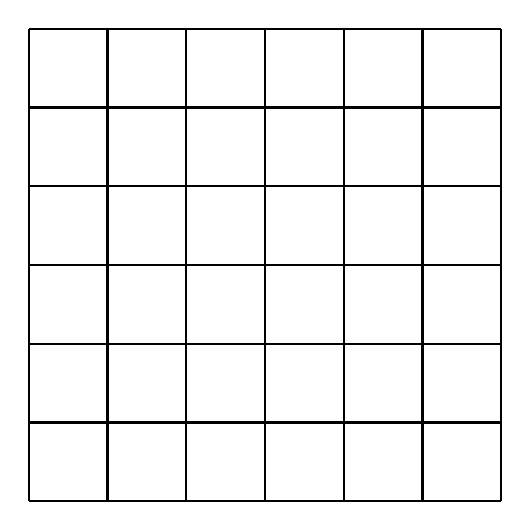
\begin{tikzpicture}
	% Draw the grid
	\draw[step=1,black,thick] (0,0) grid (6,6);
	% Draw arrows on the planes
	\drawarrow{1}{1}{0}
	\drawarrow{2}{1}{1}
	\drawarrow{3}{1}{1}
	\drawarrow{4}{1}{0}
	\drawarrow{5}{1}{0}
	\drawarrow{6}{1}{1}
	
	\drawarrow{1}{2}{0}
	\drawarrow{2}{2}{1}
	\drawarrow{3}{2}{1}
	\drawarrow{4}{2}{0}
	\drawarrow{5}{2}{1}
	\drawarrow{6}{2}{1}
	
	\drawarrow{1}{3}{1}
	\drawarrow{2}{3}{0}
	\drawarrow{3}{3}{0}
	\drawarrow{4}{3}{1}
	\drawarrow{5}{3}{0}
	\drawarrow{6}{3}{1}
	
	\drawarrow{1}{4}{1}
	\drawarrow{2}{4}{0}
	\drawarrow{3}{4}{0}
	\drawarrow{4}{4}{1}
	\drawarrow{5}{4}{1}
	\drawarrow{6}{4}{0}
	
	\drawarrow{1}{5}{1}
	\drawarrow{2}{5}{1}
	\drawarrow{3}{5}{0}
	\drawarrow{4}{5}{1}
	\drawarrow{5}{5}{0}
	\drawarrow{6}{5}{0}
	
	\drawarrow{1}{6}{0}
	\drawarrow{2}{6}{1}
	\drawarrow{3}{6}{0}
	\drawarrow{4}{6}{0}
	\drawarrow{5}{6}{0}
	\drawarrow{6}{6}{1}
	
	
\end{tikzpicture}
			\end{center}}
		\end{column}
	\end{columns}
\end{frame}

\begin{frame}{Example: Ferromagnetism}
	\begin{columns}
		\begin{column}{0.5\textwidth}
			Energy classical Ising model:
			\begin{enumerate}
				\pause
				\item \textbf{Decreases} if neighbouring magnets point in \textbf{same} direction.
				\pause
				\item \textbf{Increases} if neighbouring magnets point in \textbf{different} direction.
				\pause
				\item Formula:\[E=-J\sum_{<i,j>}\sigma_i\sigma_j\]
			\end{enumerate}
		\end{column}
		\begin{column}{0.5\textwidth}
			\begin{center}
				\newcommand{\drawarrow}[3]{
\ifnum#3=0
	\node at (#1-0.5, #2-0.5) {{\color{blue}$\uparrow$}};
\fi
\ifnum#3=1
\node at (#1-0.5, #2-0.5) {{\color{red}$\downarrow$}};
\fi

}
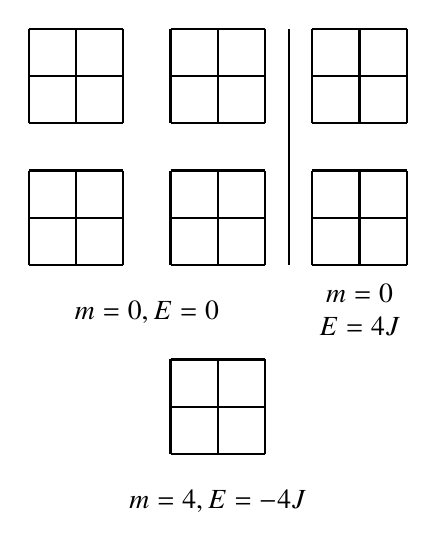
\begin{tikzpicture}[scale=0.6]
	% Draw the grid
	\newcommand\numX{0};
	\newcommand\numY{0};
	\draw[step=1,black,thick] (\numX,\numY) grid (\numX+2,\numY+2);
	\drawarrow{1+\numX}{1+\numY}{0};
	\drawarrow{2+\numX}{1+\numY}{0};
	\drawarrow{1+\numX}{2+\numY}{1};
	\drawarrow{2+\numX}{2+\numY}{1};
	
	\renewcommand\numX{3};
	\renewcommand\numY{0};
	\draw[step=1,black,thick] (\numX,\numY) grid (\numX+2,\numY+2);
	\drawarrow{1+\numX}{1+\numY}{0};
	\drawarrow{2+\numX}{1+\numY}{1};
	\drawarrow{1+\numX}{2+\numY}{0};
	\drawarrow{2+\numX}{2+\numY}{1};
	
	\renewcommand\numX{0};
	\renewcommand\numY{3};
	\draw[step=1,black,thick] (\numX,\numY) grid (\numX+2,\numY+2);
	\drawarrow{1+\numX}{1+\numY}{1};
	\drawarrow{2+\numX}{1+\numY}{1};
	\drawarrow{1+\numX}{2+\numY}{0};
	\drawarrow{2+\numX}{2+\numY}{0};
	
	\renewcommand\numX{3};
	\renewcommand\numY{3};
	\draw[step=1,black,thick] (\numX,\numY) grid (\numX+2,\numY+2);
	\drawarrow{1+\numX}{1+\numY}{1};
	\drawarrow{2+\numX}{1+\numY}{0};
	\drawarrow{1+\numX}{2+\numY}{1};
	\drawarrow{2+\numX}{2+\numY}{0};
	
	\node at (2.5,-1) {$m=0,E=0$};
	
	\renewcommand\numX{6};
	\renewcommand\numY{0};
	\draw[step=1,black,thick] (\numX,\numY) grid (\numX+2,\numY+2);
	\drawarrow{1+\numX}{1+\numY}{1};
	\drawarrow{2+\numX}{1+\numY}{0};
	\drawarrow{1+\numX}{2+\numY}{0};
	\drawarrow{2+\numX}{2+\numY}{1};
	
	\renewcommand\numX{6};
	\renewcommand\numY{3};
	\draw[step=1,black,thick] (\numX,\numY) grid (\numX+2,\numY+2);
	\drawarrow{1+\numX}{1+\numY}{0};
	\drawarrow{2+\numX}{1+\numY}{1};
	\drawarrow{1+\numX}{2+\numY}{1};
	\drawarrow{2+\numX}{2+\numY}{0};
	
	\node at (7,-1) {$\begin{matrix}
			m=0\\E=4J
		\end{matrix}$};
	
	\renewcommand\numX{3};
	\renewcommand\numY{-4};
	\draw[step=1,black,thick] (\numX,\numY) grid (\numX+2,\numY+2);
	\drawarrow{1+\numX}{1+\numY}{0};
	\drawarrow{2+\numX}{1+\numY}{0};
	\drawarrow{1+\numX}{2+\numY}{0};
	\drawarrow{2+\numX}{2+\numY}{0};
	
	\node at (4,-5) {$m=4,E=-4J$};
	
	\draw[step=1,black,thick] (5.5,0) -- (5.5,5);
\end{tikzpicture}
			\end{center}
		\end{column}
	\end{columns}
\end{frame}

\begin{frame}{Example: Ferromagnetism}
	\begin{columns}
		\begin{column}{0.5\textwidth}
			Entropy classical Ising model:
			\begin{enumerate}
				\item $n$ is amount of configurations with a given $m$.
				\item Entropy is:
				\[S=\log(n).\]
				\pause
			\end{enumerate}
		\end{column}
		\begin{column}{0.5\textwidth}
			\begin{center}
				\newcommand{\drawarrow}[3]{
\ifnum#3=0
	\node at (#1-0.5, #2-0.5) {{\color{blue}$\uparrow$}};
\fi
\ifnum#3=1
\node at (#1-0.5, #2-0.5) {{\color{red}$\downarrow$}};
\fi

}
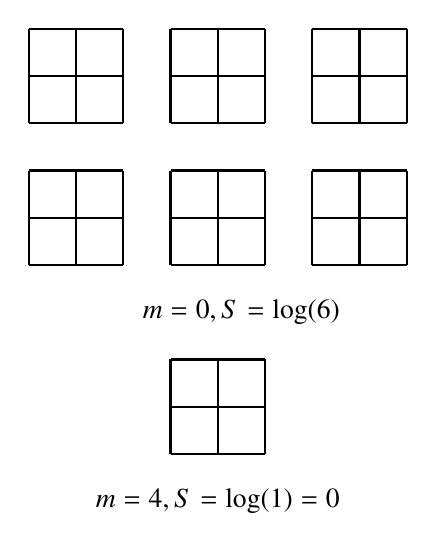
\begin{tikzpicture}[scale=0.6]
	% Draw the grid
	\newcommand\numX{0};
	\newcommand\numY{0};
	\draw[step=1,black,thick] (\numX,\numY) grid (\numX+2,\numY+2);
	\drawarrow{1+\numX}{1+\numY}{0};
	\drawarrow{2+\numX}{1+\numY}{0};
	\drawarrow{1+\numX}{2+\numY}{1};
	\drawarrow{2+\numX}{2+\numY}{1};
	
	\renewcommand\numX{3};
	\renewcommand\numY{0};
	\draw[step=1,black,thick] (\numX,\numY) grid (\numX+2,\numY+2);
	\drawarrow{1+\numX}{1+\numY}{0};
	\drawarrow{2+\numX}{1+\numY}{1};
	\drawarrow{1+\numX}{2+\numY}{0};
	\drawarrow{2+\numX}{2+\numY}{1};
	
	\renewcommand\numX{0};
	\renewcommand\numY{3};
	\draw[step=1,black,thick] (\numX,\numY) grid (\numX+2,\numY+2);
	\drawarrow{1+\numX}{1+\numY}{1};
	\drawarrow{2+\numX}{1+\numY}{1};
	\drawarrow{1+\numX}{2+\numY}{0};
	\drawarrow{2+\numX}{2+\numY}{0};
	
	\renewcommand\numX{3};
	\renewcommand\numY{3};
	\draw[step=1,black,thick] (\numX,\numY) grid (\numX+2,\numY+2);
	\drawarrow{1+\numX}{1+\numY}{1};
	\drawarrow{2+\numX}{1+\numY}{0};
	\drawarrow{1+\numX}{2+\numY}{1};
	\drawarrow{2+\numX}{2+\numY}{0};
	
	\node at (4.5,-1) {$m=0,S=\log(6)$};
	
	\renewcommand\numX{6};
	\renewcommand\numY{0};
	\draw[step=1,black,thick] (\numX,\numY) grid (\numX+2,\numY+2);
	\drawarrow{1+\numX}{1+\numY}{1};
	\drawarrow{2+\numX}{1+\numY}{0};
	\drawarrow{1+\numX}{2+\numY}{0};
	\drawarrow{2+\numX}{2+\numY}{1};
	
	\renewcommand\numX{6};
	\renewcommand\numY{3};
	\draw[step=1,black,thick] (\numX,\numY) grid (\numX+2,\numY+2);
	\drawarrow{1+\numX}{1+\numY}{0};
	\drawarrow{2+\numX}{1+\numY}{1};
	\drawarrow{1+\numX}{2+\numY}{1};
	\drawarrow{2+\numX}{2+\numY}{0};
	
	\renewcommand\numX{3};
	\renewcommand\numY{-4};
	\draw[step=1,black,thick] (\numX,\numY) grid (\numX+2,\numY+2);
	\drawarrow{1+\numX}{1+\numY}{0};
	\drawarrow{2+\numX}{1+\numY}{0};
	\drawarrow{1+\numX}{2+\numY}{0};
	\drawarrow{2+\numX}{2+\numY}{0};
	
	\node at (4,-5) {$m=4,S=\log(1)=0$};
\end{tikzpicture}
			\end{center}
		\end{column}
	\end{columns}
\end{frame}

\begin{frame}{Example: Ferromagnetism}
	\begin{columns}
		\begin{column}{0.5\textwidth}
			With temperature?
			\begin{itemize}
				\item If $T\rightarrow\infty$, maximize entropy ($m=0$).
				\item If $T\rightarrow 0$, minimize energy ($m=1$ or $m=-1$).
			\end{itemize}
		\end{column}
		\begin{column}{0.5\textwidth}
			\begin{center}
				\includegraphics[width=0.8\textwidth]{Images/IsingPhaseTransition.png}
			\end{center}
		\end{column}
	\end{columns}
\end{frame}

\subsection{Ordinary phase of matter}

\begin{frame}{Landau phases of matter}
	\begin{itemize}
		\item Parameters like $m$ are called \textbf{local order parameters}.
		\item Landau paradigm gives a consistent way to construct them.
		\item All phases of matter found before 1980 are of this form.
	\end{itemize}
\end{frame}

\begin{frame}{Todo}
	\begin{itemize}
		\item[\done] Ordinary phases of matter
		\begin{itemize}
			\item[\done] Local order parameters
		\end{itemize}
		\item[\todo] Integer quantum hall effect
		\begin{itemize}
			\item[\todo] Hall effect
			\item[\todo] Hall plateaus
			\item[\todo] No local order parameters
		\end{itemize}
		\item[\todo] Topological phases of matter
		\begin{itemize}
			\item[\todo] Low temperature?
			\item[\todo] How robust?
			\item[\todo] Topological?
		\end{itemize}
		\item[\todo] Symmetry protected topological phases of matter
		\begin{itemize}
			\item[\todo] Short range entangled
			\item[\todo] Symmetry
		\end{itemize}
		\item[\todo] Results
	\end{itemize}
\end{frame}

\section{Topological phases of matter}

\begin{frame}{Lorenz Force}
	\begin{center}
		\includegraphics[width=0.7\textwidth]{Images/Lorentz_force.pdf}
	\end{center}
\end{frame}

\subsection{Hall effect}

\begin{frame}{Hall effect}
	\begin{center}
		\includegraphics[width=0.8\textwidth]{Images/HallEffect.png}
	\end{center}
	\pause
	\begin{itemize}
		\item Keep $I$ fixed and vary $B$.
		\item Keep track of $R_x=V_x/I$, $R_H=V_H/I$.
	\end{itemize}
\end{frame}

\begin{frame}{Hall effect}
	\begin{itemize}
		\item Keep $I$ fixed and vary $B$.
		\item Keep track of $R_x=V_x/I$, $R_H=V_H/I$.
	\end{itemize}
	\pause
	 For normal temperatures and normal magnetic fields:
	\begin{center}
		\includegraphics[width=0.6\textwidth]{Images/ClassicalHallResistance.png}
	\end{center}
\end{frame}

\subsection{Integer quantum hall effect}

\begin{frame}{Integer quantum hall effect}
	\begin{columns}
		\begin{column}{0.7\textwidth}
			\begin{center}
				\includegraphics[width=\textwidth]{Images/IntegerQHE.png}
			\end{center}
		\end{column}
		\begin{column}{0.3\textwidth}
			\begin{itemize}
				\item In 1980
				\item Klaus Von Klitzing
				\item Silicon based MOSFET
				\item Very low temperatures (liquid Helium).
				\item Very high magnetic fields.
			\end{itemize}
		\end{column}
	\end{columns}
\end{frame}

\begin{frame}{Integer quantum hall effect}
	\begin{columns}
		\begin{column}{0.7\textwidth}
			\begin{center}
				\includegraphics[width=\textwidth]{Images/IntegerQHE.png}
			\end{center}
		\end{column}
		\begin{column}{0.3\textwidth}
			On plateau exactly (up to one part in a billion):
			\[R_H=\frac{c}{i}\qquad \begin{matrix}
			c=\frac{h}{e^2}\\i=\text{ integer.}
			\end{matrix}\]
			\pause
			Robust/independent under:
			\begin{itemize}
				\item Magnetic field.
				\item Disorder.
				\item Choice of material/doping.
			\end{itemize}
		\end{column}
	\end{columns}
\end{frame}

\begin{frame}{Integer quantum hall effect}
	\begin{itemize}
		\item Robust discrete property of material.
		\pause
		\item Is it phase of matter (just like gas, liquid, solid or magnetized)?
		\pause
		\item
		Local order parameter?
	\end{itemize}
\end{frame}

\begin{frame}{Integer quantum hall effect}
	From semiclassical arguments: Current distribution:
	\begin{center}
		\includegraphics[width=0.8\textwidth]{Images/HallEffectSemiclassicalCurrents.png}
	\end{center}
	\pause
	No local order. Yet global hall resistance is quantized.
\end{frame}

\begin{frame}{Todo}
	\begin{itemize}
		\item[\done] Ordinary phases of matter
		\begin{itemize}
			\item[\done] Local order parameters
		\end{itemize}
		\item[\done] Integer quantum hall effect
		\begin{itemize}
			\item[\done] Hall effect
			\item[\done] Hall plateaus
			\item[\done] No local order parameters
		\end{itemize}
		\item[\todo] Topological phases of matter
		\begin{itemize}
			\item[\todo] Low temperature?
			\item[\todo] How robust?
			\item[\todo] Topological?
		\end{itemize}
		\item[\todo] Symmetry protected topological phases of matter
		\begin{itemize}
			\item[\todo] Short range entangled
			\item[\todo] Symmetry
		\end{itemize}
		\item[\todo] Results
	\end{itemize}
\end{frame}

\subsection{Definition}

\begin{frame}{Topological phases of matter}
	\begin{block}{Definition}
		A phase of matter is topological if it has no local order parameters.
	\end{block}
	\pause
	Examples:
	\begin{itemize}
		\item Invertible topological order
		\begin{itemize}
			\item like integer quantum hall plateau/Chern insulator
		\end{itemize}
		\item Anyonic topological order
		\begin{itemize}
			\item like fractional quantum hall effect/Toric code
		\end{itemize}
	\end{itemize}
	\pause
	Questions:
	\begin{enumerate}
		\item Why low temperature?
		\item How robust?
		\item Topological?
	\end{enumerate}
\end{frame}

\section{Building model for topological phases of matter}

\subsection{Quantum phases of matter}
\begin{frame}{Unique gapped groundstates}
	What do all topological phases of matter have in common?
	\pause
	\begin{columns}
		\begin{column}{0.7\textwidth}
			They are described by Hamiltonians $H$ that
			\begin{itemize}
				\item<3-> have a "unique gapped (bulk) ground-state" $\ket{\psi}$.
				\item<4-> are a sum of local terms.
			\end{itemize}
		\end{column}
		\begin{column}{0.3\textwidth}
			\begin{center}
				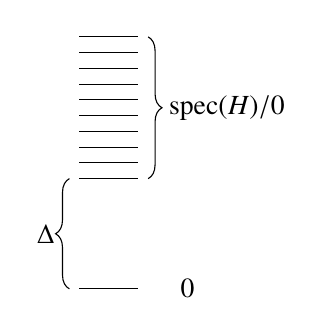
\begin{tikzpicture}
	\node (1L) at (0,0) {};
	\node (1R) at (1,0) {};
	\draw (1L) -- (1R);
	\foreach \i in {2,...,11}
	{
		\node (\i L) at (0,1+0.2*\i) {};
		\node (\i R) at (1,1+0.2*\i) {};
		\draw (\i L) -- (\i R);
	}
	\node[] (1Groundstate) at (1.5,0) {$0$};
	\draw [decorate,decoration={brace,amplitude=5pt},xshift=0cm,yshift=0pt] (0,0) -- (0,1.4) node [black,midway,xshift=-0.3cm] {$\Delta$};
	\draw [decorate,decoration={brace,amplitude=5pt},xshift=0cm,yshift=0pt] (1,1+0.2*11) -- (1,1.4)  node [black,midway,xshift=1cm] {$\textrm{spec}(H)/0$};
\end{tikzpicture}
			\end{center}
		\end{column}
	\end{columns}
	\onslide<5->{Topological order only depends on groundstate.\\
		Other (excited) states do not have it.}
	
	
\end{frame}

\begin{frame}{Connected states}
	Two states $\ket{\psi_0}$ and $\ket{\psi_1}$ are connected if
	\begin{center}
		\begin{tikzpicture}
		\node (0) [circle,fill,inner sep=3pt] at (0,0) {};
		\node (0 -1) [] at (0,-0.5) {$\ket{\psi_0}$};
		\node (1) [circle,fill,inner sep=3pt] at (5,0) {};
		\node (1 -1) [] at (5,-0.5) {$\ket{\psi_1}$};
		\draw [line width=2pt,-{Stealth[scale = 1.2]}] (0) -- (1);
		\node (arrow) [] at (2.5,-0.5) {$\ket{\psi_t}$};
		\end{tikzpicture}
	\end{center}
	where $\ket{\psi_t}$, satisfies a Shr\"odinger equation:
	\[i\partial_t\ket{\psi_t}=\sum_{i\in\Lambda} K_{i}(t) \ket{\psi_t}\]
	for some local generators $K_i(t)$.
\end{frame}

\begin{frame}{Gapped Phases Of Quantum Matter}
	\begin{center}
		\includegraphics[width=\textwidth]{Images/GappedPhasesOfQuantumMatter.pdf}
	\end{center}
	\pause
	\textbf{Topological indices are robust over each gapped phase of matter.}
\end{frame}

\subsection{Topology}

\begin{frame}{Detour: Winding number}
	\begin{center}
		\includegraphics[width=0.6\textwidth]{Images/1200px-Winding_Number_Around_Point.svg.png}
	\end{center}
	Move and shrink rope but no knots.\\
	\pause
	Goal: Find obstruction to shrinking the rope to a point.
\end{frame}

\begin{frame}{Detour: Winding number}
	\begin{center}
		\includegraphics[width=0.8\textwidth]{Images/Winding-numbers-for-several-closed-oriented-curves-In-each-case-the-winding-number-is.png}
	\end{center}
\end{frame}

\begin{frame}{Detour: Winding number}
	In mathematics language: Calculate homotopy classes of maps
	\[\vec h:\TT\rightarrow\RR^2\setminus\{0\}:k\mapsto \vec h(k).\]
	\pause
	Winding number:
	\begin{align*}
		w(\hat{h})=&\frac{1}{2\pi} c(\hat{h})&c&=\int\d k \: \hat{z}\cdot \left(\hat{h}(k)\times \partial_k \hat{h}(k)\right)
	\end{align*}
	\begin{itemize}
		\item $\hat{h}(k)$ is unit vector.
		\item $c$ is circumference of $\hat{h}$.
	\end{itemize}
	 
\end{frame}

\begin{frame}{Detour 2: Wrapping number}
	Same but in 3d.\\
	\pause
	Can't draw this.\\
	\pause
	Calculate homotopy classes of maps
	\[\vec h:\TT^2\rightarrow \RR^3\setminus \{0\}:(k_1,k_2)\mapsto \vec{h}(k_1,k_2).\]
	\pause
	Has wrapping:
	\begin{align*}
		W(\hat{h})&=\frac{1}{4\pi}S(\hat{h})&S&=\int \d^2 k \: \hat{h}\times \left(\partial_{k_1}\hat{h}\times \partial_{k_2}\hat{h}\right)
	\end{align*}
	\begin{itemize}
		\item $\hat{h}(k)$ is unit vector.
		\item $S$ is surface area of $\hat{h}$.
	\end{itemize}
\end{frame}

\begin{frame}{Topological?}
	Why is integer quantum hall effect (IQHE) topological?
	\pause
	\begin{itemize}
		\item Given a model with IQHE, there is an $\vec h:\TT^2\rightarrow \RR^3\setminus\{0\}$.
		\pause
		\item It has hall resistance $R_H=\frac{h}{e^2}\frac{1}{W(\hat h)}$.
		\pause
		\item Smooth deformations of groundstate lead to smooth deformations of $\vec h$.
	\end{itemize}
	\pause
	Wrapping number is example of an \textbf{index}.
	\pause
	\begin{block}{Definition:}
		Indices are discrete numbers that protect topological phases of matter.
	\end{block}
\end{frame}

\begin{frame}{Todo}
	\begin{itemize}
		\item[\done] Ordinary phases of matter
		\begin{itemize}
			\item[\done] Local order parameters
		\end{itemize}
		\item[\done] Integer quantum hall effect
		\begin{itemize}
			\item[\done] Hall effect
			\item[\done] Hall plateaus
			\item[\done] No local order parameters
		\end{itemize}
		\item[\done] Topological phases of matter
		\begin{itemize}
			\item[\done] Low temperature?
			\item[\done] How robust?
			\item[\done] Topological?
		\end{itemize}
		\item[\todo] Symmetry protected topological phases of matter
		\begin{itemize}
			\item[\todo] Short range entangled
			\item[\todo] Symmetry
		\end{itemize}
		\item[\todo] Results
	\end{itemize}
\end{frame}

\section{Extending topological phases of matter using symmetry}
\begin{frame}{Scope of the rest of the talk}
	\begin{center}
		\includegraphics[width=\textwidth]{Images/TrivialGappedPhaseOfQuantumMatter.pdf}
	\end{center}
	\textbf{What is the trivial phase?}
\end{frame}

\subsection{Short range entanglement}

\begin{frame}{Connected states (again)}
	Two states $\ket{\psi_0}$ and $\ket{\psi_1}$ are connected if
	\begin{center}
		\begin{tikzpicture}
			\node (0) [circle,fill,inner sep=3pt] at (0,0) {};
			\node (0 -1) [] at (0,-0.5) {$\ket{\psi_0}$};
			\node (1) [circle,fill,inner sep=3pt] at (5,0) {};
			\node (1 -1) [] at (5,-0.5) {$\ket{\psi_1}$};
			\draw [line width=2pt,-{Stealth[scale = 1.2]}] (0) -- (1);
			\node (arrow) [] at (2.5,-0.5) {$\ket{\psi_t}$};
		\end{tikzpicture}
	\end{center}
	where $\ket{\psi_t}$, satisfies a Shr\"odinger equation:
	\[i\partial_t\ket{\psi_t}=\sum_{i\in\Lambda} K_{i}(t) \ket{\psi_t}\]
	for some local generators $K_i(t)$.
\end{frame}

\begin{frame}{Short range entanglement (SRE)}
	\begin{tikzpicture}
	\foreach \i in {1,...,11}
	{
		\node[circle,fill,inner sep=1.5pt] (\i) at (\i,0) {};
		
	}
	\node[] (i) at (6,0.5) {$i$};
	\node[] (i+1) at (7,0.5) {$i+1$};
	\node[] (i+2) at (8,0.5) {$i+2$};
	\draw [decorate,decoration={brace,amplitude=5pt},xshift=0cm,yshift=0pt] (5+0.3,-0.3) -- (5-0.3,-0.3) node [black,midway,yshift=-0.3cm] {\footnotesize $\CC^d$};
	
	
\end{tikzpicture}
	\begin{block}{Definition: Product state}
		$\ket{\phi}$ is a product state if it is of the form $\bigotimes_{i\in\Lambda}\ket{v_i}$.
	\end{block}
	\pause
	\textbf{State with no entanglement.}
	\pause
	\begin{block}{Definition: short range entangled (SRE)}
		$\ket{\psi}$ is SRE if it is connected to a product state.
	\end{block}
	\pause
	\textbf{State where entanglement is short.}
\end{frame}

\begin{frame}{Endow with symmetry}
	\begin{center}
		\includegraphics[width=\textwidth]{Images/G-invariant_Parts_Of_SRE_Phase.pdf}
	\end{center}
\end{frame}


\section{Symmetry}

\begin{frame}{Symmetry}
	\begin{enumerate}
		\item A group $G$.
		\item A space $S$.
		\item A representation $R$.
		\item Invariant elements $s\in S$.
	\end{enumerate}
\end{frame}

\subsection{Symmetry: Example 1}

\begin{frame}{Example 1: Mirror symmetry}
	\begin{columns}
		\begin{column}{0.6\textwidth}
			\begin{center}
				\includegraphics[width=0.6\textwidth]{Images/symmetry_shapes.png}
			\end{center}
		\end{column}
		\begin{column}{0.4\textwidth}
			\begin{itemize}
				\item $G=\ZZ_2=\{1,-1\}$.
				\item $S$ is space of two dimensional shapes.
				\item $R(1)$ is trivial.
				\item $R(-1)$ mirrors the shape.
				\item To the left are shown six invariant shapes.
			\end{itemize}
		\end{column}
	\end{columns}
\end{frame}

\subsection{Symmetry: Example 2}

\begin{frame}{$U(1)$ representation of $U(1)$}
	\begin{columns}
		\begin{column}{0.6\textwidth}
			\begin{center}
				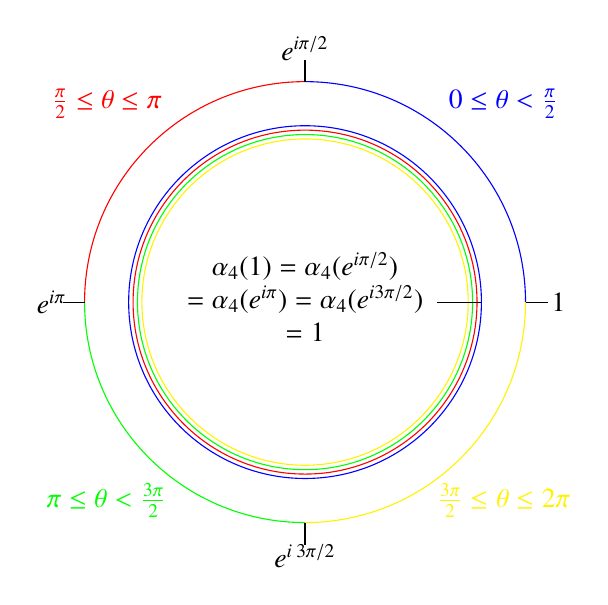
\begin{tikzpicture}
\newcommand{\s}{2.8}

% Draw the curves of the four quadrants of a circle in different colors
\draw[blue] (\s,0) arc (0:90:\s);
\draw[red] (0,\s) arc (90:180:\s);
\draw[green] (-\s,0) arc (180:270:\s);
\draw[yellow] (0,-\s) arc (270:360:\s);

% Draw a circle at the center (0,0)
\draw[blue] (0,0) circle (0.8*\s);
\draw[red] (0,0) circle (0.78*\s);
\draw[green] (0,0) circle (0.76*\s);
\draw[yellow] (0,0) circle (0.74*\s);

\draw (\s,0) -- (\s*1.1,0);
\node at (\s*1.15,0) {$1$};

\draw (0,\s) -- (0,\s*1.1);
\node at (0,\s*1.15) {$e^{i\pi/2}$};

\draw (-\s,0) -- (-\s*1.1,0);
\node at (-\s*1.15,0) {$e^{i\pi}$};

\draw (0,-\s) -- (0,-\s*1.1);
\node at (0,-\s*1.15) {$e^{i\: 3\pi/2}$};

\draw (0.8*\s,0)--(0.6*\s,0);
\node at (0,0) {$\begin{matrix}
	\alpha_4(1)=\alpha_4(e^{i\pi/2})\\
	=\alpha_4(e^{i\pi})=\alpha_4(e^{i3\pi/2})\\
	=1
	\end{matrix}$};

% Add labels
\node at (0.9*\s,0.9*\s) {\color{blue}\(0 \leq \theta < \frac{\pi}{2}\)};
\node at (-0.9*\s,0.9*\s) {\color{red}\(\frac{\pi}{2} \leq \theta \leq \pi\)};
\node at (-0.9*\s,-0.9*\s) {\color{green}\(\pi \leq \theta < \frac{3\pi}{2}\)};
\node at (0.9*\s,-0.9*\s) {\color{yellow}\(\frac{3\pi}{2} \leq \theta \leq 2\pi\)};

\end{tikzpicture}
			\end{center}
		\end{column}
		\begin{column}{0.4\textwidth}
			\begin{itemize}
				\item $q\in\ZZ$ (integer).
				\item A representation $\alpha_q\in\hom(U(1),U(1))$ is of the form
				\begin{equation*}
					\alpha_q:e^{i\theta}\mapsto e^{iq\theta}.
				\end{equation*}
				\item We call $q$ the charge.
			\end{itemize}
		\end{column}
	\end{columns}
\end{frame}

\begin{frame}{Example 2: Electric charge in quantum mechanics}
\begin{columns}
	\begin{column}{0.4\textwidth}
		\begin{center}
			\includegraphics[width=\textwidth]{Images/Bloch_sphere.pdf}
		\end{center}
	\end{column}
	\begin{column}{0.6\textwidth}
		\begin{itemize}
			\item Vector space $V=\CC^2$ with two basis vectors $\ket{0}$ and $\ket{1}$.
			\item For any $\ket{v}\in V$ we can write
			\[\ket{\Psi(\theta,\phi)}=\sin(\theta)\ket{0}+e^{i\phi}\cos(\theta)\ket{1}.\]
			\pause
			\item $R=\alpha_{q_1}\oplus\alpha_{q_2}$. So
			\begin{align*}
			R(e^{i\psi})\ket{0}&=\alpha_{q_1}(e^{i\psi})\ket{0}=e^{i q_1 \psi}\ket{0}\\
			R(e^{i\psi})\ket{1}&=\alpha_{q_2}(e^{i\psi})\ket{1}=e^{i q_2 \psi}\ket{1}.
			\end{align*}
			\pause
			\item This means that
			\[R(e^{i\psi})\ket{\Psi(\theta,\phi)}=\ket{\Psi(\theta,\phi+(q_2-q_1)\psi)}.\]
			\item Only $\ket{0}$ and $\ket{1}$ are invariant.
		\end{itemize}
	\end{column}
\end{columns}
\end{frame}

\begin{frame}{Example 2: Electric charge in quantum mechanics}
	\begin{block}{Consequence}
		In a $U(1)$ invariant, isolated quantum mechanical system, only states with the same charge are connected.
	\end{block}
	\pause
	\begin{itemize}
		\item The generalization of this to general $G$ is called the 0-D symmetry protected topological (or SPT) classification.
		\pause
		\item It is classified by $\alpha\in\hom(G,U(1))$.
		\pause
		\item What is the generalization of this to higher dimensions?
	\end{itemize}
\end{frame}

\section{SPT classification}

\begin{frame}{On site group action}
	\textbf{Representation in 1D:}\\$\:$\\
	\pause
	\scalebox{0.8}{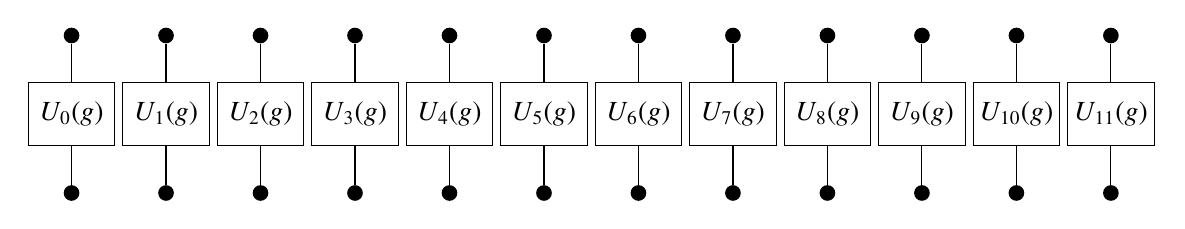
\begin{tikzpicture}
	\foreach \x in {0,...,11}{
		\node (\x) [circle,fill,inner sep=2pt] at (\x*1.2,0) {};
		\node (2\x) [] at (\x*1.2,-1) {};
		\node (3\x) [circle,fill,inner sep=2pt] at (\x*1.2,-2) {};
	}
	
	\foreach \x in {0,...,11}{
		\draw (\x) -- (2\x);
		\draw (2\x) -- (3\x);
	}
	
	\foreach \x in {0,...,11}
	\draw [fill=white] (\x*1.2-0.55,-0.6) rectangle (\x*1.2+0.55,-1.40);
	
	\foreach \x in {0,...,11}{
		\node (other \x) [] at (\x*1.2,-1) {$U_{\x}(g)$};
	}
\end{tikzpicture}}
	\pause
	\begin{align*}
		U(g)&=\bigotimes_{i\in\Lambda}U_i(g)&U_i\in&\hom(G,U(\CC^d)).
	\end{align*}
	\pause
	\textbf{$G$-Invariant state:}
	\[U(g)\ket{\psi}\propto\ket{\psi}.\]
\end{frame}

\begin{frame}{On site group action}
	\textbf{A path:}\\
	\begin{equation*}
		\begin{tikzpicture}
			\node (0) [circle,fill,inner sep=3pt] at (0,0) {};
			\node (0 -1) [] at (0,-0.5) {$\ket{\psi_0}$};
			\node (1) [circle,fill,inner sep=3pt] at (5,0) {};
			\node (1 -1) [] at (5,-0.5) {$\ket{\psi_1}$};
			\draw [line width=2pt,-{Stealth[scale = 1.2]}] (0) -- (1);
			\node (arrow) [] at (2.5,-0.5) {$\ket{\psi_t}$};
			\node at (9,0) {$i\partial_t\ket{\psi_t}=\sum_{i\in\Lambda}K_i \ket{\psi_t}$};
		\end{tikzpicture}
	\end{equation*}
	is $G$-invariant if
	\[[K_i,U(g)]=0\]
	for each $i\in\Lambda$.
\end{frame}

\begin{frame}
	\begin{center}
		\includegraphics[width=\textwidth]{Images/SPT_Phases.pdf}
	\end{center}
\end{frame}

\begin{frame}{Todo}
	\begin{itemize}
		\item[\done] Ordinary phases of matter
		\begin{itemize}
			\item[\done] Local order parameters
		\end{itemize}
		\item[\done] Integer quantum hall effect
		\begin{itemize}
			\item[\done] Hall effect
			\item[\done] Hall plateaus
			\item[\done] No local order parameters
		\end{itemize}
		\item[\done] Topological phases of matter
		\begin{itemize}
			\item[\done] Low temperature?
			\item[\done] How robust?
			\item[\done] Topological?
		\end{itemize}
		\item[\done] Symmetry protected topological phases of matter
		\begin{itemize}
			\item[\done] Short range entangled
			\item[\done] Symmetry
		\end{itemize}
		\item[\todo] Results
	\end{itemize}
\end{frame}

\begin{frame}{SPT index}
	A map
	\[\textrm{index}:\{\psi\text{ is SRE and $G$-invariant}\}\rightarrow\{\textrm{discrete set}\}\]
	is an SPT index if
	\begin{align*}
		\psi_1&\sim_G\psi_2&&\Rightarrow&\textrm{index}(\psi_1)&=\textrm{index}(\psi_2).
	\end{align*}
	\pause
	An SPT index is complete if $\Leftrightarrow$.
\end{frame}

\section{Results}

\begin{frame}{1D SPT classification results}
	Let $\AA$ be a quasi local algebra over $\ZZ$.
	\begin{block}{Theorem 1:}
		There exists an $H^2(G,U(1))$ valued index on $G$-invariant SRE states. This index is invariant under $G$-invariant LGA's\footnote{Yoshiko Ogata. A classification of pure states on quantum spin chains satisfying the split property with on-site finite group symmetries. arXiv:1908.08621, 2019.}. (This result is more general)
	\end{block}
\end{frame}

\begin{frame}{1D SPT classification results}
	Let $\AA$ be a quasi local algebra over $\ZZ$.
	\begin{block}{Theorem 2:}
		If two $G$-invariant SRE states $\omega_1$ and $\omega_2$ have the same $H^2(G,U(1))$-valued index then there exist $G$-invariant product states $\phi_1,\phi_2$ and an LGA $\gamma_{0;1}^K$ such that
		\[\omega_1\otimes_{\text{stack}}\phi_1=\omega_2\otimes_{\text{stack}}\phi_2\circ\gamma_{0;1}^K \footnote{Anton Kapustin, Nikita Sopenko, and Bowen Yang. A classification of invertible phases of bosonic quantum lattice systems in one dimension. Journal of Mathematical Physics, 62(8):081901, Aug 2021.}.\]
	\end{block}
\end{frame}

\begin{frame}{Loops of 1D SPT classification results}
	Let $\AA$ be a quasi local algebra over $\ZZ$.
	\begin{block}{Theorem 3:}
		$G$-invariant locally generated loops of invertible states are classified by an $H^2(G,U(1))\oplus H^1(G,U(1))$-valued index. This classification is also complete.\footnote{Sven Bachmann, Wojciech De Roeck, Martin Fraas and Tijl Jappens, A classification of G-charge Thouless pumps in 1D invertible states, https://doi.org/10.48550/arxiv.2204.03763, 2022}
	\end{block}
\end{frame}

\begin{frame}{2D SPT classification results}
	Let $\AA$ be a quasi local algebra over $\ZZ^2$.
	\begin{block}{Theorem 4:}
		$G$-invariant SRE's carry an $H^3(G,U(1))$-valued index. This index is invariant under $G$-invariant LGAs.\footnote{Yoshiko Ogata. A $H^3(G,U(1))$-valued index of symmetry protected topological phases with on-site finite group symmetry for two-dimensional quantum spin systems. arXiv:2101.00426, 2021.}
	\end{block}
\end{frame}

\begin{frame}{2D translation invariant SPT classification results}
	Let $\AA$ be a quasi local algebra over $\ZZ^2$.
	\begin{block}{Theorem 5:}
		$G$-invariant stably SRE's, that are translation invariant in one direction carry an $H^3(G,U(1))\oplus H^2(G,U(1))$-valued index. This index is invariant under $G$-invariant, translation invariant LGA's.\footnote{Tijl Jappens, SPT indices emerging from translation invariance in two-dimensional quantum spin systems, https://doi.org/10.48550/arxiv.2202.11758, 2022}
	\end{block}
\end{frame}

\begin{frame}{2D translation invariant SPT classification results}
	Let $\AA$ be a quasi local algebra over $\ZZ^2$.
	\begin{block}{Theorem 6:}
		$G$-invariant stably SRE's, that are translation invariant in two directions carry an
		\[H^3(G,U(1))\oplus H^2(G,U(1))\oplus H^2(G,U(1))\oplus H^1(G,U(1))\]
		-valued index. This index is invariant under $G$-invariant, translation invariant (in two directions) LGA's.\footnote{Tijl Jappens, SPT indices emerging from translation invariance in two-dimensional quantum spin systems, https://doi.org/10.48550/arxiv.2202.11758, 2022 (Accepted by CMP).}
	\end{block}
\end{frame}

\section{End slide}

\begin{frame}{Todo}
	\begin{itemize}
		\item[\done] Ordinary phases of matter
		\begin{itemize}
			\item[\done] Local order parameters
		\end{itemize}
		\item[\done] Integer quantum hall effect
		\begin{itemize}
			\item[\done] Hall effect
			\item[\done] Hall plateaus
			\item[\done] No local order parameters
		\end{itemize}
		\item[\done] Topological phases of matter
		\begin{itemize}
			\item[\done] Low temperature?
			\item[\done] How robust?
			\item[\done] Topological?
		\end{itemize}
		\item[\done] Symmetry protected topological phases of matter
		\begin{itemize}
			\item[\done] Short range entangled
			\item[\done] Symmetry
		\end{itemize}
		\item[\done] Results
	\end{itemize}
\end{frame}

\begin{frame}{End of the presentation}
	\begin{center}
		\includegraphics[width=0.8\textwidth]{Images/thank-you.png}
	\end{center}
\end{frame}

\end{document}